\documentclass{article}
\usepackage{arxiv}

\usepackage[utf8]{inputenc}
\usepackage[english, russian]{babel}
\usepackage[T1]{fontenc}
\usepackage{url}
\usepackage{booktabs}
\usepackage{amsfonts}
\usepackage{amsmath}
\usepackage{nicefrac}
\usepackage{microtype}
\usepackage{lipsum}
\usepackage{subcaption}
\usepackage{graphicx}
\usepackage{natbib}
\usepackage{doi}
\usepackage{color}
\usepackage{xcolor}

\newcommand{\TODO}[1]{\textcolor{purple}{ToDo: #1.}}

\title{Binary Neural Networks. Lossless picture quality for binary neural networks in pixel-level tasks.}

\author{Kirill Ovcharenko \\
	Moscow Institute of Physics and Technology\\
	%% examples of more authors
	\And
	Zharikov Ilya \\
	Moscow Institute of Physics and Technology\\
	%% \AND
	%% Coauthor \\
	%% Affiliation \\
	%% Address \\
	%% \texttt{email} \\
	%% \And
	%% Coauthor \\
	%% Affiliation \\
	%% Address \\
	%% \texttt{email} \\
	%% \And
	%% Coauthor \\
	%% Affiliation \\
	%% Address \\
	%% \texttt{email} \\
}
\date{}

\renewcommand{\shorttitle}{\textit{arXiv} Template}

%%% Add PDF metadata to help others organize their library
%%% Once the PDF is generated, you can check the metadata with
%%% $ pdfinfo template.pdf
\hypersetup{
pdftitle={A template for the arxiv style},
pdfsubject={q-bio.NC, q-bio.QM},
pdfauthor={David S.~Hippocampus, Elias D.~Striatum},
pdfkeywords={First keyword, Second keyword, More},
}

\begin{document}
\maketitle

\begin{abstract}
Image Super Resolution [SR] is a crucial class of image processing techniques that enhance quality of visual data. 
Deep Convolutional Neural Networks [DCNN] have recently shown great results in this field. However, application of DCNN on resource-limited devices remains challenging, as they demand significant amounts of memory, energy and computations. Binary neural networks [BNN] provide a promising approach to reduce computational complexity and speed up the inference of a model. To our best knowledge, there are not many papers devoted to applying BNN to SR tasks, as SR models are much more vulnerable to degradation in performance when decreasing the precision of weights, than image classification models. The paper proposes modification of a convolutional block to make it binary without performance decreasing.

\end{abstract}


\keywords{Binary Neural Network \and Single Image Super Resolution \and Binarization \and Model compression}

\section{Introduction}

\TODO{Need to be extended in terms related works further}

Image Super Resolution [SR] aims to restore High Quality [HQ] image from corrupted Low Quality [LQ] counterpart. This task is important because of its various applications in medical imaging and surveillance instruments. In spite of the research in this field being active, it made some progress not a long ago, as some challenges were encountered. Main obstacle is desired output in SR tasks being much more diverse than input, so the model is required to do dense pixel-level prediction, hence is bound to be more complex.  

Recent advances in the field of SR owe their success to Deep Neural Networks [DNN] which show state-of-the-art results in a wide range of computer vision problems, such as image classification, Semantic Segmentation etc. However, the models solving these tasks are usually complicated and demand a lot of space and computational resources, thus hindering their implementation on mobile devices, drones and other machines which are limited in GPU memory.

Lately, different methods of reducing complexity of these models were proposed. While some papers focus on pruning and knowledge distillation, other researches introduce quantization as a way to decrease memory needed.

The most extreme form of quantization is binarization. Binary Neural Networks [BNN] use only $1$ bit to represent each parameter, thus drastically decreasing space demanded to store the model. Moreover, with all parameters of the model set to $\{-1, 1\}$, most of the the calculations can be conducted using XNOR and Bitcount operations. This approach seems promising, as it proposes new ways to design hardware that can help to handle and exploit complex neural networks.

However, it is obvious that BNN sacrifice precision and quality, as they have much less capacity and representational potential than Full-Precision [FP] networks. Previous works in this field propose different methods of maintaining competitive accuracy while achieving better performance. The paper~\cite{ma2019efficient} focuses on residual block binarization, which helps to reduce a significant part of the model's parameters. However, full-precision activations keep computational complexity of the model pretty high. ReactNet~\cite{liu2020reactnet} suggests generalized binarization and activations functions that help to shift distribution, which significantly increases representational capacity of the binary model. The BBCU~\cite{xia2022basic} proposed effective Convolutional Unit that can be used in any architecture that relies on residual connections. It provides much more efficient training and inference, but oversimplifies weight binarization. IR-Net~\cite{qin2020forward} reduces information loss by balancing weights to achieve maximum information entropy in forward propagation. After that, IR2Net~\cite{xue2022ir2net} proposes two essential components of the learning process: Information Restriction and Information Recovery. BNext~\cite{guo2022join} also applies attention mechanism to obtain the key information from the full-precision activations and smooth out the loss landscape. 
However, last two papers investigate only the impact of these methods on performance of Image Classification models. Another way of extracting necessary information was proposed in~\cite{hu2018squeeze}, where a squeeze-and-excitation block is added to every transformation to a feature map, so that it can learn dependencies between channels (which are expected to concentrate on different features). In contrast to regular approaches, the paper~\cite{zhao2020efficient} presented a new method of attention that helps model to better get pixel-level dependencies and exhibits great results in SR task.

This paper adopts some techniques from the researches, mentioned above, and suggests further modifications of convolutional block that help to improve BNN's performance in SR tasks.

We use EDSR~\cite{lim2017enhanced} as a backbone for our modified binary block, as it doesn't require batch normalization module and shows state-of-the-art results. We use BBCU~\cite{xia2022basic} as a baseline for our modification as it showed prominent performance in multiple Image Restoration tasks, particularly in SR. This paper proposes several adjustments for the binary convolutional block.

Firstly, we adopt the idea of using generalized activation and sign functions from \cite{liu2020reactnet}. That helps to achieve better performance while preserving reasonable computational demands. 

Secondly, we keep the idea of updating full-precision weights with respect to binarized weights from ~\cite{ma2019efficient}. We also maintain a learnable scale factor in contrast to ~\cite{xia2022basic}, where the optimal value is used, because the former method was proven to give better results.

Finally, we advance the idea from ~\cite{xue2022ir2net} and ~\cite{guo2022join} to restrict information from the input to increase learning productivity by implementing attention modules into our binary network. We try different ways to compute attention maps, including the methods proposed in ~\cite{zhao2020efficient} and ~\cite{hu2018squeeze}.

\section{Problem statement}
\label{sec:headings}

\TODO{Need to be slightly reformulated during theory week}

Let $\{(X_i, Y_i)\}_{i=1}^n$ be our image dataset, where $X_i \in \mathbb{R}^{h_i \times w_i \times 3}$ denotes the low resolution image and $Y_i \in \mathbb{R}^{H_i \times W_i \times 3}$ - the high resolution one. Considering $M$ to be the model, SR task targets optimization of 
\begin{equation}
    Q(M) = \frac{1}{n}\sum\limits_{i=1}^nf(M(X_i), Y_i)
\end{equation}
where $f$ represents either $PSNR$ or $SSIM$ metric, defined as:
\begin{equation}
    PSNR(x, y) = 10 \log_{10} \left(\frac{MAX_I^2}{MSE(x, y)}\right)
\end{equation}


Here $MAX_I$ is the maximum valid value for pixel, $MSE$ is mean squared error.

\begin{equation}
    SSIM(x, y) = \frac{(2\mu_x\mu_y + c_1)(2\sigma_{xy} + c_2)}{(\mu_x^2 + \mu_y^2 + c_1)(\sigma_{x}^2 + \sigma_{y}^2 + c_2)}
\end{equation}

$\mu_x$ denotes the mean for $x$, $\mu_y$ is the mean for $y$, $\sigma_x$ is the variance for $x$, $\sigma_y$ is the variance for $y$, $\sigma_{xy}$ is the covariation of $x$ and $y$, $c_1$ and $c_2$ - two constants depending on dynamic pixel range.

Now let $B \in \mathcal{B}$ be our binarized representation of model $M$. $\mathcal{B}$ is space of BNN. Assuming $L$ to be number of layers in $B \in \mathcal{B}$, $W_l \in \{-1, 1\}^{C_{out} \times C_{in} \times K_h \times K_w}$, $l \in \{1 \ , ... \ , L\}$. Here $C_{out}$ is the number of output channels, $C_{in}$ is the number of input channels, $K_h$ is the kernel height, $K_w$ is the kernel weight. 


Thus, the problem of binarization can be expressed in finding $B^{*}$ as
\begin{equation}
    B^{*} = \arg\min\limits_{B \in \mathcal{B}} \left[Q(M) - Q(B)\right]
\end{equation}

\section{Basic Binary Convolutional Block modification}
\subsection{Baseline block}

In this section we define basic binarization operations that are used to build the Binary Convolutional Block.

Let $X_t^f \in \mathbb{R}^{H \times W \times C_{in}}$ and $W_t^f \in \mathbb{R}^{K_{h} \times K_{w} \times C_{in} \times C_{out}}$ be full-precision activations and full-precision convolution weights on the $t$-th layer respectively. Here $H$ and $W$ denote the input feature map height and width, $C_{in}$ stands for the number of input channels and $C_{out}$ is the number of output channels. Then $X_t^b \in \{-1, 1\}^{H \times W \times C_{in}}$, $W_t^b \in \{-1, 1\}^{\times K_{w} \times C_{in} \times C_{out}}$ would be the binary approximations for the corresponding full-precision parameters.

When using binary parameters, convolution operation $X^b \ast W^b$ can be effectively performed using XNOR and Bitcount operations:

\begin{equation*}
    X_t^b \ast W_t^b = Bitcount(XNOR(X_t^b, W_t^b))
\end{equation*}

We adopt the idea of using generalized sign function from ~\cite{liu2020reactnet}, as it was proven to help BNNs better learn distributions of activations. Thus, the binary representations can be acquired by applying RSign function:

\begin{equation}
    x_{i, j, k}^b = RSign(x_{i, j, k}^f) = 
    \begin{cases}
        +1, & x_{i, j, k}^f > \alpha_k \\
        -1, & x_{i, j, k}^f \le \alpha_k 
    \end{cases}, \quad
    i \in [0, H), j \in [0, W), k \in [0, C_{in})
\label{eq_act_sign}
\end{equation}

Here $x_{i, j, k}^f \in X_t^f$, $x_{i, j, k}^b \in X_t^b$ are single full-precision and binary activations respectively.

When binarizing the convolution weights we use the regular Sign function:

\begin{equation}
    w_{i, j, k, l}^b = Sign(w_{i, j, k, l}^f) = 
    \begin{cases}
        +\alpha_l, & w_{i, j, k, l}^f > 0 \\
        -\alpha_l, & w_{i, j, k, l}^f \le 0
    \end{cases}, \quad
    i \in [0, H), j \in [0, W), k \in [0, C_{in}), l \in [0, C_{out})
\end{equation}

Here full-precision and binary weights are denoted as $w_{i, j, k, l}^f \in W_t^f$, $w_{i, j, k, l}^b \in W_t^b$.

We preserve the idea from ~\cite{ma2019efficient} of using learnable $\alpha_l$ parameter instead of the optimal value $\alpha_l = \dfrac{|W_l|}{n}$, as optimality in the optimisation task is not necessary consistent with the optimality of target loss function.

We use RPReLU~\cite{liu2020reactnet} as activation function, because it achieves better performance by shifting the negative component of input's distribution, which is important for BNNs.

RPReLU is defined as follows:

\begin{equation}
    RPReLU(x_{i, j, k}) = 
    \begin{cases}
        x_{i, j, k} - \gamma_{k} + \zeta_{k}, & x_{i, j, k} > \gamma_{k} \\
        \beta_k(x_{i, j, k} - \gamma_k) + \zeta_k, & x_{i, j, k} \le \gamma_k
    \end{cases}, \quad
    i \in [0, H), j \in [0, W), k \in [0, C_{in})
\end{equation}

Where $x_{i, j, k} \in \mathbb{R}^{H \times W \times C_{in}}$ is an element of the input feature map, $\gamma_i \in \mathbb{R}$ and $\zeta_i \in \mathbb{R}$ are learnable shifts for moving the distribution, and $\beta_i \in \mathbb{R}$ is a learnable coefficient controlling the slope of the negative part.

Previous researches displayed the importance of the residual connection in the Binary Convolution Block, especially in the SR task, so we keep it for every binary convolution to transfer the full-precision information through the block. Moreover, BBCU~\cite{xia2022basic} shows that activation function narrows the negative part of the residual connection, thus losing negative full-precision information. On that account, we keep the idea of moving the residual connection out of the activation function.

EDSR~\cite{lim2017enhanced} showed that applying Batch Normalization has a negative impact on quality when dealing with pixel-level tasks, such as SR. But the experiments conducted in ~\cite{xia2022basic} show that spreading the distribution of values is necessary for BNNs. For that reason, we adopt the amplification factor from BBCU~\cite{xia2022basic} that helps to avoid covering the full-precision information with the binary convolution output. 

Taking in consideration all the points mentioned above, the baseline block can be expressed as follows:

\begin{equation}
    X_{t+1}^f = RPReLU(X_{t}^b \ast W_t^b) + kX_t^f
\end{equation}

Here $X_{t}^b$ was also acquired from the amplified activations $kX_t^f$, but the learnable threshold from \ref{eq_act_sign} helps to filter the amplitude. 

\subsection{Attention modules}
When the full-precision model is being binarized, it is bound to lose some representational capacity and suffer a performance decrease. Previous researches~\cite{guo2022join, xue2022ir2net} focus on applying attention mechanism to help the model to capture the most important features and dependencies. Further advancing the idea of restricting information, we suggest attention modules that help the model to extract necessary features from the input. 

We propose several different attention blocks: a simple squeeze-and-excitation attention, a spatial attention and a pixel attention.

A squeeze-and-excitation block~\cite{hu2018squeeze} is depicted on \ref{blocks:a}. It consists of Global Average Pooling (GAP), two linear layers with a non-linear activation function (ReLU) and a sigmoid function, which is defined as follows:

\begin{equation*}
    \sigma(x) = \dfrac{1}{1 + e^{-x}}
\end{equation*}

The structure of the block helps model to learn non-linear dependencies between channels, hence between different features.

Spatial attention block (\ref{blocks:b}) consists of one $1\times1$ convolution with $1$ output channel followed by a sigmoid function. It focuses on getting a 2D attention map which helps it to learn relationships between channels for every pixel on the feature map.

Finally, pixel attention block (\ref{blocks:c}) has similar structure to the spatial attention block, except for using a $1 \times 1$ convolution with the same number of the output channels. It constructs a 3D attention map that learn connections between both the channels and the pixels. Previous works~\cite{zhao2020efficient} proved it to be the best option for SR tasks as it helps to learn complex pixel-level dependencies.

\begin{figure}[h]
\centering
  \begin{subfigure}[c]{0.33\textwidth}
    \includegraphics[width=\linewidth]{se_attn.png}
    \caption{Squeeze-and-excitation attention} \label{blocks:a}
  \end{subfigure}%
  \hspace*{\fill}   % maximize separation between the subfigures
  \begin{subfigure}[c]{0.33\textwidth}
    \includegraphics[width=\linewidth]{spat_attn.png}
    \caption{Spatial attention block} \label{blocks:b}
  \end{subfigure}%
  \hspace*{\fill}   % maximizeseparation between the subfigures
  \begin{subfigure}[c]{0.33\textwidth}
    \includegraphics[width=\linewidth]{pixel_attn.png}
    \caption{Pixel attention block} \label{blocks:c}
  \end{subfigure}

\caption{Attention blocks} \label{blocks}
\end{figure}


\begin{figure}[h]
\label{block}
\centering
\includegraphics[width=0.8\textwidth]{block.png}
\caption{Basic binary block modification} \label{block}
\end{figure}

\subsection{Proposed modification}
In the baseline block, outputs of the binary convolution and activations from the previous layer are added to each other and have the same influence on the result. However, full-precision residual connections have information that cannot be effectively processed by the binary convolution due to its simple structure. Therefore, we need to provide a method to get the most important features from previous layer. Hence, we add an attention module to the residual branch of the convolutional block. 

However, the outputs of the convolution branch can also contain unnecessary information that should not be propagated to the next layer. Thus, we add another attention block that is applied to the RPReLU output before connecting with residual information.

To give the model more freedom when deciding on the importance of information, we add scaling factors $a_1$ and $a_2$ to the binary convolution and residual branches respectively. Having these coefficients as learnable parameters help the model to propagate the most essential features to the next layers. Moreover, tuning these coefficients alleviates the need of using amplification factor, as $a_1$ and $a_2$ can maintain necessary amplitude of distribution of the residual information.

The block with all the mentioned modifications is presented on \ref{block}. Independently constructed attention maps are applied to both residual and binary branches and the outputs are connected using learnable scaling coefficients. 

Having similar structure with BBCU, the block can be used in any SR model architecture with minimal effort. In the next section we implement the modified block into EDSR and prove it to show state-of-the-art results on the benchmark datasets.

\section{Computational experiment}
\subsection{Preliminary report}
\begin{figure}[h]
\caption{Validation metric plots for baseline (BBCU)}
\centering
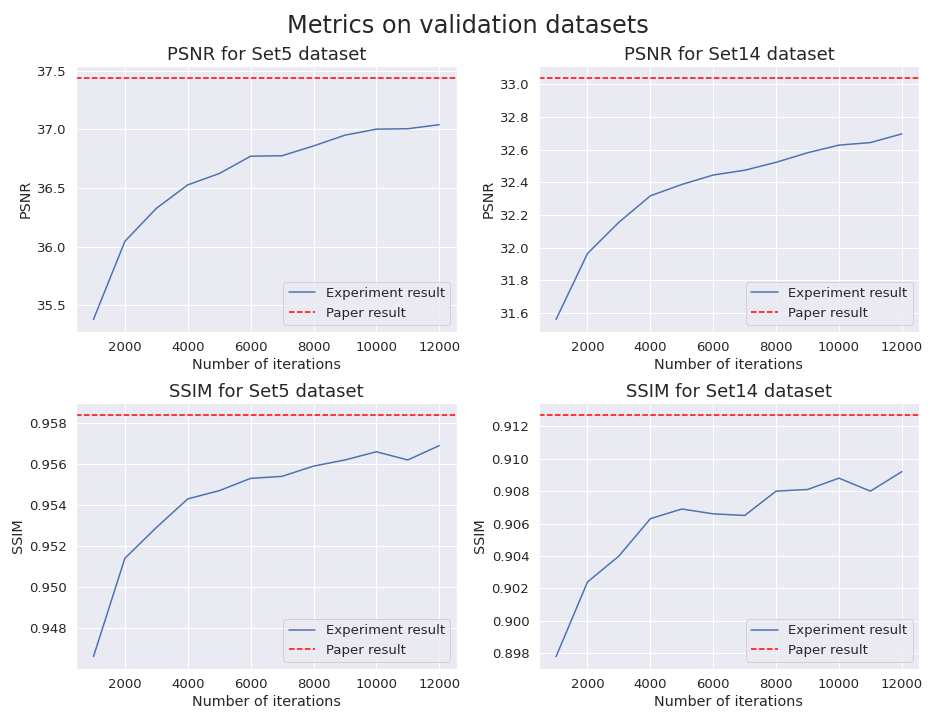
\includegraphics[width=0.8\textwidth]{val_metrics.png}
\end{figure}
We expect our modification to show the same trend of PSNR and SSIM metrics, but the goal of the research is to increase the performance while preserving the amount of computational resources required.


\bibliographystyle{unsrtnat}
\bibliography{references}

\end{document}